% Compilação: pdflatex notas_de_aula_fisica1.tex (duas vezes).
% Arquivo autossuficiente: figuras desenhadas em TikZ, sem imagens externas.
\documentclass[11pt,a4paper]{article}
\usepackage[utf8]{inputenc}
\usepackage[T1]{fontenc}
\usepackage{babel}
\babelprovide[main,import]{portuguese}
\addto\captionsportuguese{\renewcommand{\contentsname}{Sumário}}
\usepackage{lmodern,amsmath,amssymb,geometry,booktabs,array}
\usepackage{xcolor,tikz,hyperref,fancyhdr}
\usetikzlibrary{arrows.meta}
\geometry{margin=2.3cm,headheight=15pt}
\definecolor{azul}{HTML}{164B70}
\hypersetup{colorlinks=true,linkcolor=azul,urlcolor=azul,pdftitle={Física I: vetores e cinemática vetorial}}
\pagestyle{fancy}\fancyhf{}
\fancyhead[L]{\small Física I | Vetores e cinemática}
\fancyhead[R]{\small Notas de aula}
\fancyfoot[C]{\thepage}
\setlength{\parindent}{0pt}\setlength{\parskip}{6pt}
\setlength{\emergencystretch}{2em}
\allowdisplaybreaks
\newcommand{\vi}{\vec{i}}\newcommand{\vj}{\vec{j}}\newcommand{\vk}{\vec{k}}
\newcommand{\norm}[1]{\left\lVert #1\right\rVert}
\newcommand{\alerta}[1]{\par\textbf{Atenção:} #1\par}
\title{\textcolor{azul}{\textbf{Física I}}\\Vetores e cinemática vetorial\\\large Notas de aula com deduções e exemplos da Lista 1}
\author{Material de estudo para David Abrantes}
\date{30 de setembro de 2026}
\begin{document}
\maketitle
\textbf{Base do material.} Lista 1 de Exercícios de Física 1, 2026.2, enviada pelo estudante: 20 questões de vetores, operações vetoriais e cinemática vetorial. O roteiro abaixo cobre todos os temas dessa lista. Não representa confirmação de conteúdos adicionais da professora que não estejam no documento.

\textbf{Como estudar.} Leia primeiro a ideia geométrica, acompanhe a dedução e refaça os exemplos sem olhar. Adotamos eixos cartesianos fixos e ortonormais, ângulos positivos no sentido anti-horário e $g=9{,}8\,\mathrm{m/s^2}$. Nos exercícios 12 e 16, usamos as aproximações trigonométricas exigidas pela lista. Resultados aproximados são arredondados apenas ao final.

\textbf{Conexões com seus estudos.} Componentes e versores retomam Geometria Analítica e bases da Álgebra Linear; derivadas e integrais dão significado às equações do movimento; a queda livre conecta a teoria ao experimento com vídeo e Tracker. Médias, incertezas e mínimos quadrados pertencem ao tratamento experimental e não são exigidos nesta lista.
\clearpage
\tableofcontents
\newpage
\section{Referenciais, modelos e linguagem matemática}
\textbf{Objetivo desta aula.} Entender o que precisamos escolher antes de descrever um movimento.

Imagine uma pessoa sentada em um barco que está sendo levado pela correnteza. Sua posição em relação ao barco permanece constante, mas sua posição em relação à margem muda. Portanto, dizer apenas ``está em movimento'' é incompleto: precisamos especificar um referencial.

\textbf{Definição.} Um sistema de coordenadas cartesiano associa a cada ponto uma tripla $(x,y,z)$, usando uma origem e três eixos perpendiculares. Um referencial inclui a estrutura em relação à qual medimos posições e tempos. Neste material, usamos um relógio comum da mecânica clássica e uma base cartesiana fixa.

\textbf{Modelo de partícula.} Descrevemos um corpo por um único ponto quando seu tamanho e sua rotação não são essenciais ao problema. Isso não significa que o corpo seja realmente pontual. No lançamento de uma bola, por exemplo, o modelo pode descrever sua trajetória sem explicar sua rotação.

\textbf{Unidades e dimensões.} Posição tem dimensão de comprimento, $[x]=L$; velocidade, $[v]=L/T$; aceleração, $[a]=L/T^2$. Na expressão $x=x_0+v_0t+at^2/2$, cada termo precisa ter dimensão de comprimento:
\[
[v_0t]=(L/T)T=L,\qquad [at^2]=(L/T^2)T^2=L.
\]
Só podemos somar grandezas de mesma dimensão. Esse teste detecta erros, mas não prova que uma equação esteja correta: ele não determina, por exemplo, o fator $1/2$.

\textbf{Convenção sobre as funções da lista.} Quando escrevemos $x(t)=3t^2$ com $x$ em metros e $t$ em segundos, o coeficiente 3 tem unidade $\mathrm{m/s^2}$. As unidades não desaparecem por não estarem escritas em cada coeficiente.

\textbf{Pergunta de verificação.} Se uma pessoa está parada em relação ao barco, sua velocidade em relação à margem é necessariamente zero? Não: depende da velocidade do barco em relação à margem. Retomaremos essa ideia na travessia do rio.

\section{Vetores: tamanho, direção e sentido}
Uma grandeza escalar é descrita por um número e uma unidade, como massa ou tempo. Uma grandeza vetorial precisa também de direção e sentido, como deslocamento, velocidade e força. Direção identifica a orientação da reta; sentido distingue as duas possibilidades nessa reta.

No plano, escrever $\vec A=A_x\vi+A_y\vj$ significa construir o vetor somando uma contribuição horizontal e outra vertical. Os versores $\vi$, $\vj$ e $\vk$ têm módulo 1 e apontam nos sentidos positivos dos eixos. As componentes podem ser negativas; o módulo nunca é negativo.

\begin{center}
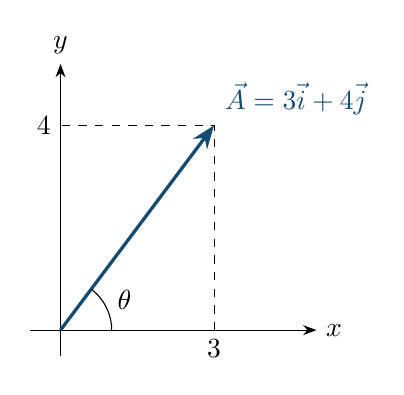
\begin{tikzpicture}[scale=.65,>=Stealth]
\draw[->](-.6,0)--(5,0)node[right]{$x$};
\draw[->](0,-.5)--(0,5.2)node[above]{$y$};
\draw[very thick,->,azul](0,0)--(3,4)node[above right]{$\vec A=3\vi+4\vj$};
\draw[dashed](3,0)node[below]{$3$}--(3,4)--(0,4)node[left]{$4$};
\draw(1,0)arc[start angle=0,end angle=53.13,radius=1];
\node at (1.25,.6){$\theta$};
\end{tikzpicture}
\end{center}
O triângulo retângulo da figura dá, por Pitágoras,
\[A^2=A_x^2+A_y^2\quad\Longrightarrow\quad \boxed{A=\norm{\vec A}=\sqrt{A_x^2+A_y^2}}.\]
Em três dimensões, aplicar Pitágoras mais uma vez fornece $A=\sqrt{A_x^2+A_y^2+A_z^2}$.

Pelas definições trigonométricas, se $\theta$ é medido desde $+x$,
\[\cos\theta=\frac{A_x}{A},\qquad \sin\theta=\frac{A_y}{A}
\quad\Longrightarrow\quad\boxed{A_x=A\cos\theta,\quad A_y=A\sin\theta}.\]
Para recuperar o ângulo, use os sinais das componentes para identificar o quadrante. A função $\operatorname{atan2}(A_y,A_x)$ faz isso automaticamente. Usar apenas $\arctan(A_y/A_x)$ pode errar o quadrante e não funciona quando $A_x=0$.

\subsection*{Exemplos da lista: questões 1 e 2}
Q1: para $(3,4)$, $A=\sqrt{3^2+4^2}=\sqrt{9+16}=5{,}00$.
Ambas as componentes são positivas: primeiro quadrante. Assim,
$\theta=\arctan(4/3)=53{,}13^\circ$. A representação é a seta da origem ao ponto $(3,4)$.

Q2: para $B=10$ e $\theta=30^\circ$,
\[B_x=10\cos30^\circ=10\frac{\sqrt3}{2}=5\sqrt3\approx8{,}66,
\qquad B_y=10\sin30^\circ=10\frac12=5{,}00.\]

\section{Soma, subtração, escalares e vetor unitário}
Somar vetores equivale a realizar dois deslocamentos consecutivos. Pode-se transladar a segunda seta para sua origem coincidir com a ponta da primeira. A resultante vai do início ao fim do percurso. Algebricamente,
\[\vec A\pm\vec B=(A_x\pm B_x)\vi+(A_y\pm B_y)\vj+(A_z\pm B_z)\vk.\]
Subtrair $\vec B$ é somar $-\vec B$. Multiplicar por $\lambda$ multiplica todas as componentes, com $\norm{\lambda\vec A}=|\lambda|\norm{\vec A}$. Se $\lambda<0$, o sentido se inverte; se $\lambda=0$, obtém-se o vetor nulo, que não tem direção definida.

Um vetor unitário tem módulo 1. Para obter o unitário com o mesmo sentido de $\vec A\ne\vec0$, dividimos cada componente pelo módulo:
\[\boxed{\hat a=\frac{\vec A}{\norm{\vec A}}},\qquad
\norm{\hat a}=\frac{\norm{\vec A}}{\norm{\vec A}}=1.\]

\subsection*{Exemplos da lista: questões 3 a 7}
\textbf{Q3.} $\vec A=(2,5)$ e $\vec B=(-3,1)$:
\[\vec A+\vec B=(2-3,5+1)=(-1,6),\qquad
\norm{\vec A+\vec B}=\sqrt{(-1)^2+6^2}=\sqrt{37}\approx6{,}08.\]
\begin{center}
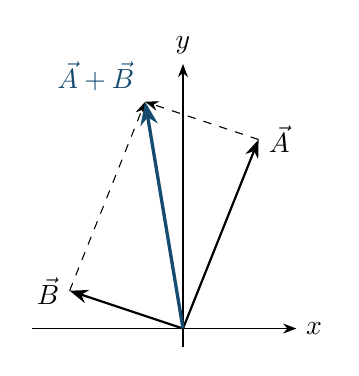
\begin{tikzpicture}[scale=.48,>=Stealth]
\draw[->](-4,0)--(3,0)node[right]{$x$};\draw[->](0,-.5)--(0,7)node[above]{$y$};
\draw[->,thick](0,0)--(2,5)node[right]{$\vec A$};
\draw[->,thick](0,0)--(-3,1)node[left]{$\vec B$};
\draw[dashed,->](2,5)--(-1,6);\draw[dashed,->](-3,1)--(-1,6);
\draw[->,very thick,azul](0,0)--(-1,6)node[above left]{$\vec A+\vec B$};
\end{tikzpicture}
\end{center}
\textbf{Q4.} $\vec A-\vec B=(4-1,-2-3)=(3,-5)$.
O módulo é $\sqrt{9+25}=\sqrt{34}\approx5{,}83$.
O vetor está no quarto quadrante: $\theta=-\arctan(5/3)=-59{,}04^\circ$, ou $300{,}96^\circ$.

\textbf{Q5.} Para $\vec A=(2,-3)$, $A=\sqrt{4+9}=\sqrt{13}$.
\begin{align*}
3\vec A&=(6,-9),&\norm{3\vec A}&=3\sqrt{13}\approx10{,}82;\\
-2\vec A&=(-4,6),&\norm{-2\vec A}&=2\sqrt{13}\approx7{,}21.
\end{align*}
O fator $-2$ dobra o tamanho e inverte o sentido, mantendo a direção da reta.

\textbf{Q6.} $\norm{(6,8)}=\sqrt{36+64}=10$, portanto
$\hat a=0{,}60\vi+0{,}80\vj$. Verificação: $\sqrt{0{,}60^2+0{,}80^2}=\sqrt{1}=1$.

\textbf{Q7.} Isolando o vetor desconhecido,
\[\vec C=-(\vec A+\vec B)=-[(5,0)+(-2,3)]=-(3,3)=(-3,-3).\]
Logo, $C=\sqrt{9+9}=3\sqrt2\approx4{,}24$. As duas componentes são negativas e iguais: $\theta=180^\circ+45^\circ=225{,}00^\circ$.
\alerta{Em geral, $\norm{\vec A+\vec B}\ne A+B$. Some as componentes primeiro; calcule o módulo depois.}

\section{Produto escalar e projeções}
O produto escalar mede o alinhamento de dois vetores e resulta em um número:
\[\boxed{\vec A\cdot\vec B=AB\cos\theta=A_xB_x+A_yB_y+A_zB_z}.\]
A expressão em componentes vem da distributividade e das relações
$\vi\cdot\vi=\vj\cdot\vj=\vk\cdot\vk=1$, enquanto produtos entre versores diferentes são nulos. Assim, ao expandir $(A_x\vi+A_y\vj+A_z\vk)\cdot(B_x\vi+B_y\vj+B_z\vk)$, somente os termos de eixos iguais sobrevivem.

Para vetores não nulos,
\[\theta=\arccos\!\left(\frac{\vec A\cdot\vec B}{AB}\right).
\]
Produto positivo indica ângulo agudo; nulo, perpendicularidade; negativo, ângulo obtuso.

A projeção escalar de $\vec A$ sobre $\vec B\ne\vec0$ é a componente assinada de $\vec A$ nessa direção:
\[A_{\parallel}=A\cos\theta=\frac{\vec A\cdot\vec B}{B}.
\]
Para transformá-la em vetor, multiplicamos pelo unitário $\vec B/B$:
\[\boxed{\operatorname{proj}_{\vec B}\vec A=\frac{\vec A\cdot\vec B}{B^2}\vec B}.\]
\textbf{Conexão:} o trabalho de uma força constante é $W=\vec F\cdot\Delta\vec r$, pois somente a componente paralela ao deslocamento contribui.

\subsection*{Exemplos da lista: questões 8 e 10}
\textbf{Q8.} Para $\vec A=(3,-1,2)$ e $\vec B=(1,4,-2)$,
\begin{align*}
\vec A\cdot\vec B&=3(1)+(-1)(4)+2(-2)=3-4-4=-5;\\
A&=\sqrt{9+1+4}=\sqrt{14},\qquad B=\sqrt{1+16+4}=\sqrt{21};\\
\cos\theta&=\frac{-5}{\sqrt{14}\sqrt{21}}=\frac{-5}{\sqrt{294}};\\
\theta&\approx106{,}95^\circ.
\end{align*}
O sinal negativo confirma que o ângulo é obtuso.

\textbf{Q10.} Para $\vec A=(5,2)$ e $\vec B=(3,4)$,
\[\vec A\cdot\vec B=5(3)+2(4)=15+8=23,\qquad B=\sqrt{9+16}=5.\]
Logo, $A_{\parallel}=23/5=4{,}60$ e
\[\operatorname{proj}_{\vec B}\vec A=\frac{23}{25}(3,4)=(2{,}76,3{,}68).\]
\alerta{A projeção escalar tem sinal. Seu valor absoluto é o comprimento da projeção. A projeção vetorial precisa apontar ao longo da reta de $\vec B$.}

\section{Produto vetorial e torque}
O produto vetorial resulta em um vetor perpendicular ao plano de $\vec A$ e $\vec B$:
\[\norm{\vec A\times\vec B}=AB\sin\theta.\]
Seu módulo é a área do paralelogramo formado pelos vetores: base $A$ vezes altura $B\sin\theta$. O sentido vem da regra da mão direita, girando os dedos de $\vec A$ para $\vec B$ pelo menor ângulo.
\begin{align*}
\vec A\times\vec B
&=\begin{vmatrix}\vi&\vj&\vk\\A_x&A_y&A_z\\B_x&B_y&B_z\end{vmatrix}\\
&=(A_yB_z-A_zB_y)\vi+(A_zB_x-A_xB_z)\vj+(A_xB_y-A_yB_x)\vk.
\end{align*}
A ordem importa: $\vec B\times\vec A=-(\vec A\times\vec B)$.
No plano $xy$, basta calcular $(A_xB_y-A_yB_x)\vk$.

O torque em relação a uma origem é $\vec\tau=\vec r\times\vec F$. Seu módulo é $rF\sin\theta$: uma força produz mais efeito de rotação quando aplicada perpendicularmente e longe do ponto de referência. O torque em torno de um eixo é a componente desse vetor ao longo do eixo.

\subsection*{Exemplos da lista: questões 9 e 19}
\textbf{Q9.} $\vec A\times\vec B=(2\vi)\times(3\vj)=6(\vi\times\vj)=6\vk$.
Módulo $6{,}00$, direção do eixo $z$, sentido positivo.

\textbf{Q19.} Adotando o eixo $z$ perpendicular ao plano,
\begin{align*}
\vec\tau&=[0{,}5(-5)-0{,}3(10)]\vk\\
&=(-2{,}5-3{,}0)\vk=-5{,}50\vk\ \mathrm{N\,m}.
\end{align*}
O módulo é $5{,}50\,\mathrm{N\,m}$. Visto do semieixo $+z$ para o plano, o sentido é horário.
\alerta{Não troque $\vec r\times\vec F$ por $\vec F\times\vec r$: isso inverte o sentido.}

\section{Equilíbrio e deslocamentos sucessivos}
Em um referencial inercial, $\sum\vec F=m\vec a$. No equilíbrio translacional, $\vec a=\vec0$, portanto a resultante é nula. Isso permite repouso ou velocidade constante. Resolva separadamente $\sum F_x=0$ e $\sum F_y=0$.

\subsection*{Questão 11: força equilibrante}
Decompondo as forças,
\begin{align*}
\vec F_1&=(10,0)\ \mathrm N;\\
\vec F_2&=(15\cos120^\circ,15\sin120^\circ)
=(-7{,}5,7{,}5\sqrt3)\ \mathrm N;\\
\vec F_3&=-(\vec F_1+\vec F_2)=(-2{,}5,-7{,}5\sqrt3)\ \mathrm N.
\end{align*}
Seu módulo é $\sqrt{(-2{,}5)^2+(-7{,}5\sqrt3)^2}=\sqrt{6{,}25+168{,}75}=\sqrt{175}\approx13{,}23\,\mathrm N$.
No terceiro quadrante, $\theta=180^\circ+\arctan(7{,}5\sqrt3/2{,}5)\approx259{,}11^\circ$.

\subsection*{Questão 12: caminhada}
Escolhendo leste como $+x$ e norte como $+y$,
\[\vec d_1=(8,0),\qquad\vec d_2=(6\cdot0{,}80,6\cdot0{,}60)=(4{,}8,3{,}6)\ \mathrm m.\]
Então $\Delta\vec r=(12{,}8,3{,}6)\,\mathrm m$,
\[\norm{\Delta\vec r}=\sqrt{12{,}8^2+3{,}6^2}=\sqrt{176{,}8}\approx13{,}30\,\mathrm m,
\quad\theta=\arctan(3{,}6/12{,}8)\approx15{,}71^\circ.\]
A direção é $15{,}71^\circ$ ao norte do leste. A distância percorrida é $8+6=14\,\mathrm m$, diferente do módulo do deslocamento.

\section{Posição, velocidade e aceleração}
O vetor posição liga a origem à partícula:
$\vec r(t)=x(t)\vi+y(t)\vj+z(t)\vk$. O deslocamento liga a posição inicial à final:
\[\Delta\vec r=\vec r(t_2)-\vec r(t_1),\qquad
\vec v_m=\frac{\Delta\vec r}{t_2-t_1}.\]
Velocidade média usa deslocamento. Rapidez média usa distância total percorrida.

Para saber a velocidade em um instante, encolhemos o intervalo:
\[\boxed{\vec v(t)=\lim_{\Delta t\to0}\frac{\vec r(t+\Delta t)-\vec r(t)}{\Delta t}=\frac{d\vec r}{dt}}.
\]
Em uma base cartesiana fixa, os versores não variam com o tempo, portanto derivamos componente por componente:
\[\vec v=x'\vi+y'\vj+z'\vk,\qquad
\boxed{\vec a=\frac{d\vec v}{dt}=\frac{d^2\vec r}{dt^2}}.
\]
A rapidez é $v=\norm{\vec v}=\sqrt{v_x^2+v_y^2+v_z^2}$. A velocidade é tangente à trajetória; aceleração mede qualquer mudança da velocidade, inclusive de direção.

\subsection*{Questões 13 a 15}
\textbf{Q13.} $\Delta t=4-1=3\,\mathrm s$ e
$\Delta\vec r=(8-2,11-3)=(6,8)\,\mathrm m$. Assim,
\[\vec v_m=\frac{(6,8)}{3}=\left(2,\frac83\right)\mathrm{m/s}
\approx(2{,}00\vi+2{,}67\vj)\ \mathrm{m/s}.\]

\textbf{Q14.} Para $\vec r=(3t^2)\vi+(2t-1)\vj$, usamos
$d(t^n)/dt=nt^{n-1}$ e a derivada de uma constante igual a zero:
\[\vec v=(3\cdot2t)\vi+(2-0)\vj=6t\vi+2\vj.\]
Em $t=2\,\mathrm s$, $\vec v=12\vi+2\vj\,\mathrm{m/s}$ e
$v=\sqrt{12^2+2^2}=\sqrt{148}\approx12{,}17\,\mathrm{m/s}$.

\textbf{Q15.} Para $\vec r=5t\vi+(4t-4{,}9t^2)\vj$,
\begin{align*}
\vec v&=5\vi+(4-2\cdot4{,}9t)\vj=5\vi+(4-9{,}8t)\vj;\\
\vec a&=0\vi-9{,}8\vj\ \mathrm{m/s^2};\\
\vec v(1)&=5\vi+(4-9{,}8)\vj=5\vi-5{,}8\vj\ \mathrm{m/s};\\
v(1)&=\sqrt{25+33{,}64}=\sqrt{58{,}64}\approx7{,}66\,\mathrm{m/s}.
\end{align*}
\alerta{Derive antes de substituir o instante. Substituir primeiro transforma a posição em constantes e apaga sua dependência temporal.}

\section{Aceleração constante: dedução por integração}
Se $\vec a$ é constante e as condições iniciais são dadas em $t=0$,
\[\frac{d\vec v}{dt}=\vec a
\quad\Longrightarrow\quad
\vec v(t)-\vec v_0=\int_0^t\vec a\,ds=\vec a t.
\]
Logo, $\boxed{\vec v(t)=\vec v_0+\vec a t}$. Integrando novamente,
\begin{align*}
\vec r(t)-\vec r_0&=\int_0^t(\vec v_0+\vec a s)\,ds\\
&=\vec v_0\int_0^t ds+\vec a\int_0^t s\,ds\\
&=\vec v_0t+\tfrac12\vec a t^2.
\end{align*}
Portanto, $\boxed{\vec r(t)=\vec r_0+\vec v_0t+\tfrac12\vec a t^2}$.
Essas fórmulas exigem aceleração constante; com aceleração variável, mantenha as integrais.

\subsection*{Questão 20}
Substituindo $\vec r_0=\vec0$, $\vec v_0=(3,5)$ e $\vec a=(2,-4)$,
\[\vec v(t)=(3+2t)\vi+(5-4t)\vj,\qquad
\vec r(t)=(3t+t^2)\vi+(5t-2t^2)\vj.
\]
Em $t=3\,\mathrm s$,
\begin{align*}
\vec v(3)&=(3+6,5-12)=(9,-7)\ \mathrm{m/s};\\
v(3)&=\sqrt{81+49}=\sqrt{130}\approx11{,}40\,\mathrm{m/s};\\
\vec r(3)&=(9+9,15-18)=(18,-3)\ \mathrm m;\\
\norm{\vec r(3)}&=\sqrt{324+9}=\sqrt{333}\approx18{,}25\,\mathrm m.
\end{align*}
O último resultado é a distância à origem. A distância percorrida exigiria $\int_0^3\norm{\vec v(t)}\,dt$.

\section{Lançamento oblíquo e queda livre}
Sem resistência do ar e com gravidade uniforme, $\vec a=-g\vj$. Se o lançamento ocorre da origem, $v_{0x}=v_0\cos\theta$ e $v_{0y}=v_0\sin\theta$; as equações anteriores dão
\begin{align*}
x(t)&=v_{0x}t,& y(t)&=v_{0y}t-\tfrac12gt^2;\\
v_x(t)&=v_{0x},&v_y(t)&=v_{0y}-gt.
\end{align*}
Os movimentos horizontal e vertical compartilham o mesmo tempo, mas têm acelerações diferentes.

\textbf{Tempo de subida.} No topo, $v_y=0$, portanto
$0=v_{0y}-gt_s\Rightarrow t_s=v_{0y}/g$.

\textbf{Altura máxima acima do lançamento.} Substituindo esse tempo,
\[H=v_{0y}\frac{v_{0y}}g-\frac g2\left(\frac{v_{0y}}g\right)^2
=\frac{v_{0y}^2}{g}-\frac{v_{0y}^2}{2g}=\frac{v_{0y}^2}{2g}.\]
\textbf{Tempo de voo até a mesma altura.} Fazendo $y(T)=0$,
\[0=v_{0y}T-\tfrac12gT^2=T(v_{0y}-gT/2).
\]
Uma raiz é o lançamento, $T=0$; a outra é $T=2v_{0y}/g$.

\textbf{Alcance nessa condição.}
\[L=v_{0x}T=\frac{2v_0^2\sin\theta\cos\theta}{g}
=\frac{v_0^2\sin(2\theta)}{g}.\]
Se o impacto ocorre em altura diferente, determine $T$ resolvendo
$y_f=y_0+v_{0y}T-gT^2/2$, e depois use $L=v_{0x}T$.

\subsection*{Questão 16}
A lista não especifica a altura de chegada. Para obter tempo total e alcance, adotamos retorno ao nível do lançamento. Usando as aproximações indicadas,
$v_{0x}=20(0{,}60)=12\,\mathrm{m/s}$ e $v_{0y}=20(0{,}80)=16\,\mathrm{m/s}$.
\begin{align*}
T&=\frac{2(16)}{9{,}8}=\frac{32}{9{,}8}\approx3{,}27\,\mathrm s;\\
H&=\frac{16^2}{2(9{,}8)}=\frac{256}{19{,}6}\approx13{,}06\,\mathrm m;\\
L&=12\frac{32}{9{,}8}=\frac{384}{9{,}8}\approx39{,}18\,\mathrm m;\\
\vec v(1)&=12\vi+(16-9{,}8)\vj=12\vi+6{,}20\vj\ \mathrm{m/s};\\
v(1)&=\sqrt{144+38{,}44}=\sqrt{182{,}44}\approx13{,}51\,\mathrm{m/s};\\
\phi&=\arctan(6{,}2/12)\approx27{,}32^\circ\text{ acima da horizontal}.
\end{align*}
\alerta{No topo, somente $v_y$ se anula. A velocidade horizontal continua e a aceleração ainda é $-g\vj$.}

\textbf{Conexão com Tracker.} Em uma queda a partir do repouso, escolhendo $+y$ para cima,
$y(t)=y_0-gt^2/2$. Um ajuste $y=At^2+Bt+C$ ideal fornece $A=-g/2$, $B=v_{0y}$ e $C=y_0$. O sinal de $A$ depende do eixo escolhido. Na coleta, solta-se a esfera, registra-se o vídeo e rastreiam-se as posições; as equações entram na análise dos dados.

\subsection*{Da função horária à equação da trajetória}
As funções $x(t)$ e $y(t)$ dizem onde a partícula está em cada instante. A trajetória descreve o conjunto de pontos visitados. Para eliminar o tempo, suponha $v_{0x}\ne0$:
\[
x=v_{0x}t\quad\Longrightarrow\quad t=\frac{x}{v_{0x}}.
\]
Substituindo em $y=v_{0y}t-gt^2/2$,
\[
y=\frac{v_{0y}}{v_{0x}}x-\frac{g}{2v_{0x}^2}x^2
=x\tan\theta-\frac{g}{2v_0^2\cos^2\theta}x^2.
\]
Esta é uma parábola com concavidade para baixo. A ligação com Geometria Analítica é direta: uma equação quadrática descreve a forma da trajetória, enquanto a parametrização pelo tempo descreve também como ela é percorrida.

\textbf{Ligação com máximos e mínimos.} No topo, $y'(t)=v_y(t)=0$ e $y''(t)=-g<0$. O teste da segunda derivada confirma que a altura é máxima. Observe a diferença: $y'(t)=0$ não exige $x'(t)=0$.

\section{Movimento circular uniforme}
Uniforme significa rapidez constante. A direção da velocidade muda, logo há aceleração. Adotamos rotação anti-horária em torno da origem e $\theta(t)=\omega t$, com ângulos em radianos. A geometria do círculo dá
\[\vec r(t)=R\cos(\omega t)\vi+R\sin(\omega t)\vj.
\]
Pela regra da cadeia, $d[\cos(\omega t)]/dt=-\omega\sin(\omega t)$ e
$d[\sin(\omega t)]/dt=\omega\cos(\omega t)$. Portanto,
\begin{align*}
\vec v(t)&=-R\omega\sin(\omega t)\vi+R\omega\cos(\omega t)\vj;\\
v&=\sqrt{R^2\omega^2\sin^2(\omega t)+R^2\omega^2\cos^2(\omega t)}
=R|\omega|;\\
\vec a(t)&=-R\omega^2\cos(\omega t)\vi-R\omega^2\sin(\omega t)\vj
=-\omega^2\vec r(t).
\end{align*}
Como $\vec r$ aponta do centro para a partícula, $-\omega^2\vec r$ aponta para o centro. Seu módulo é $a_c=R\omega^2=v^2/R$. Também $\vec r\cdot\vec v=0$, confirmando a tangência da velocidade.

\subsection*{Questão 17}
Com $R=2\,\mathrm m$ e $\omega=3\,\mathrm{rad/s}$,
\begin{align*}
\vec r(t)&=2\cos(3t)\vi+2\sin(3t)\vj\ \mathrm m;\\
\vec v(t)&=-6\sin(3t)\vi+6\cos(3t)\vj\ \mathrm{m/s};\\
v&=\sqrt{36(\sin^2(3t)+\cos^2(3t))}=6{,}00\,\mathrm{m/s};\\
\vec a(t)&=-18\cos(3t)\vi-18\sin(3t)\vj\ \mathrm{m/s^2};\\
\vec a&=-9\vec r,\qquad a_c=18{,}00\,\mathrm{m/s^2}.
\end{align*}
Em $t=0$, posição $2\vi$, velocidade $6\vj$ e aceleração $-18\vi$: direita, cima e esquerda, respectivamente.
\alerta{Aceleração centrípeta não é uma força adicional: a resultante das forças existentes deve fornecer a aceleração radial.}

\section{Velocidade relativa e travessia de rio}
No regime clássico, em referenciais com eixos paralelos e sem rotação relativa,
$\vec r_{B/M}=\vec r_{B/A}+\vec r_{A/M}$. Derivando,
\[\boxed{\vec v_{B/M}=\vec v_{B/A}+\vec v_{A/M}}.
\]
Os índices indicam barco ($B$), água ($A$) e margem ($M$). É essencial saber em relação a quê cada velocidade foi medida.

\subsection*{Questão 18}
Leste é $+x$; norte é $+y$. Logo,
\[\vec v_{B/M}=4\vj+2\vi=(2\vi+4\vj)\ \mathrm{m/s}.
\]
O módulo é $\sqrt{2^2+4^2}=\sqrt{20}\approx4{,}47\,\mathrm{m/s}$.
A direção é $\arctan(4/2)=63{,}43^\circ$ ao norte do leste, ou $26{,}57^\circ$ a leste do norte.

Para cruzar a largura, usamos a componente norte: $200=4t$, então $t=200/4=50{,}00\,\mathrm s$.
A deriva é $\Delta x=v_xt=2(50)=100{,}00\,\mathrm m$ para leste.
\alerta{Dividir a largura por $4{,}47$ seria incorreto: essa rapidez corresponde ao trajeto diagonal, não à direção perpendicular às margens.}

\section{Roteiro de resolução e revisão}
\begin{enumerate}
\item Desenhe os eixos e declare os sentidos positivos.
\item Identifique se cada dado é posição, deslocamento, velocidade, aceleração ou força.
\item Decomponha os vetores na mesma base e confira as unidades.
\item Escolha a operação: soma para resultantes; produto escalar para ângulo/projeção; produto vetorial para torque; derivada para obter velocidade/aceleração; integral para reconstruir o movimento.
\item Resolva simbolicamente antes de substituir os números, quando possível.
\item Calcule o módulo somente após determinar as componentes.
\item Confira quadrante, unidade, condições da fórmula e plausibilidade física.
\end{enumerate}

\begin{center}\small
\begin{tabular}{p{.37\textwidth}p{.49\textwidth}}
\toprule Pergunta & Ferramenta central \\ \midrule
Quanto mede o vetor? & $\sqrt{A_x^2+A_y^2+A_z^2}$ \\
Qual é o unitário? & $\vec A/\norm{\vec A}$, se $\vec A\ne0$ \\
Qual é o ângulo entre vetores? & $\cos\theta=(\vec A\cdot\vec B)/(AB)$ \\
Qual é a projeção vetorial? & $(\vec A\cdot\vec B)\vec B/B^2$ \\
Qual é a velocidade? & $\vec v=d\vec r/dt$ \\
Qual é a aceleração? & $\vec a=d\vec v/dt$ \\
Como mover com $\vec a$ constante? & $\vec r=\vec r_0+\vec v_0t+\vec a t^2/2$ \\
Como combinar referenciais? & Somar velocidades com índices compatíveis \\
\bottomrule
\end{tabular}\end{center}

\textbf{Teste sua compreensão.} Explique sem consultar: (1) por que uma volta completa pode ter deslocamento nulo e distância não nula; (2) por que a aceleração no topo de um lançamento não se anula; (3) por que um movimento com rapidez constante pode ter aceleração; (4) por que a correnteza altera a deriva, mas não o tempo da questão 18; (5) por que torque e produto escalar têm resultados de naturezas diferentes.

\textbf{Respostas esperadas.} (1) O deslocamento depende apenas dos extremos. (2) A gravidade continua atuando. (3) A direção da velocidade pode mudar. (4) A correnteza é paralela às margens e não altera a componente de travessia no modelo adotado. (5) O torque é definido por um produto vetorial e tem orientação; o produto escalar fornece um número associado ao alinhamento.
\end{document}
